%1
\documentclass[a4paper,11pt]{article}
\pdfoutput=1 % if your are submitting a pdflatex (i.e. if you have
             % images in pdf, png or jpg format)

\usepackage{jinstpub} % for details on the use of the package, please
                     % see the JINST-author-manual
\usepackage{lineno}
\usepackage{epstopdf}
\usepackage{wrapfig}
\usepackage{subfig}
\usepackage{graphicx}
\title{\boldmath A search for Lepton Flavor Violating Decays of the Higgs Boson }
\proceeding{Oral Candidacy Exam proposal:\\
  Dated 24th of March, 2017\\
  }


%% %simple case: 2 authors, same institution
%% \author{A. Uthor}
%% \author{and A. Nother Author}
%% \affiliation{Institution,\\Address, Country}

% more complex case: 4 authors, 3 institutions, 2 footnotes
\author[a]{Nabarun Dev}

% The "\note" macro will give a warning: "Ignoring empty anchor..."
% you can safely ignore it.

% The "\note" macro will give a warning: "Ignoring empty anchor..."
% you can safely ignore it.

\affiliation[a]{Department of physics, University of Notre Dame, Indiana, USA}

% e-mail addresses: only for the forresponding author
\emailAdd{nabarun.dev@cern.ch, ndev@nd.edu}

\notoc
\compress
%\toccont
\abstract{A proposal is presented here outlining the search for lepton flavor violating (LFV) decays of the Higgs boson using the CMS experiment at the LHC. This a search for physics beyond the standard model and is performed with events where the Higgs decays to a muon and a tau lepton with the tau further decaying to an electron. About 36 $fb^{-1}$ of data collected by the CMS in 2016 will be used to perform this search. The signal for which we are searching, the backgrounds and the experimental techniques used to discrimate signal from background are outlined in this proposal.}





\begin{document}
%\setpagewiselinenumbers
\linenumbers

\maketitle
\flushbottom

\section{Introduction}
\label{sec:intro}
%For internal references use label-refs: see section~\ref{sec:intro}.
The Standard Model (SM) of particles physics is the most well-tested and elegant description of nature available today. 
The discovery of the Higgs Boson in 2012 ~\cite{a} added another feather in the hat of the SM.
In the SM, elementary particles acquire mass from their interaction with the scalar Higgs field, the quantum of which is the  Higgs Boson.
Besides confirming the above mechanism by which particles acquire mass, the above discovery is also significant beause the Higgs provides a portal for us to not only further study the processes within the SM, but also to look for new physics processes beyond it (BSM). 
One of the main goals of the LHC  physics programme at CERN is to search for such BSM processes.


Lepton flavour violating (LFV) interactions between charged leptons cannot naturally occur within the standard model and such a process has never been observed experimentally.
However, such decays are allowed in many BSM theories such as models with more than one Higgs doublet ~\cite{b}, supersymmetric models,~\cite{c} and many others. 
Such interactions could thus be an indicator of new physics and could be realized in decays of the Higgs Boson into two charged leptons of different flavor.
Indirect constraints on LFV Higgs decays exists through interpretations of measurements of processes such as $\tau \rightarrow \mu \gamma$~\cite{d}.
These constraints set weak limits on such decays allowing significant branching fractions;$Br(H\rightarrow \mu \tau)<O(10\%).$~\cite{e}. 
A search for $H\rightarrow \mu \tau$ performed with data collected by the CMS during run I of the LHC  improved the above limits by an order of magnitude to $Br(H\rightarrow \mu \tau)<O(1.51\%)$ at 95\% confidence level ~\cite{df}. Also, an excess of events with a significance of 2.4$\sigma$ was observed. This warrants us to do this search with much larger amount of data which would either lead us to confirm this excess or squash it and set much stricter limits on this process. The run II of LHC (see section~\ref{sec:lhccms})  provides us with such an opportunity to perform the search outlined in the following.   

\section{The LHC and the CMS }
\label{sec:lhccms} 
The Large Hadron Collider (LHC) is a circular particle accelerator designed to collide proton beams with a centre-of-mass energy of 14 TeV. It consists of a 27-kilometre ring of superconducting magnets with a number of accelerating structures to boost the energy of the particles along the way. Currently (run II), the LHC operating at a center-of-mass (COM) energy of 13 TeV (compared to 7 TeV in run I) and at luminosities up to $1.5 \times 10^{34} \mathrm{cm^{-2}s^{-1}}$. The Higgs production cross-section under these conditions is more than a factor 2 higher~\cite{f} than run I (see figure~\ref{fig:a}) and almost twice the amount of data (~36 $fb^{-1}$) have already been collected.     

\begin{figure}[htbp]
\centering
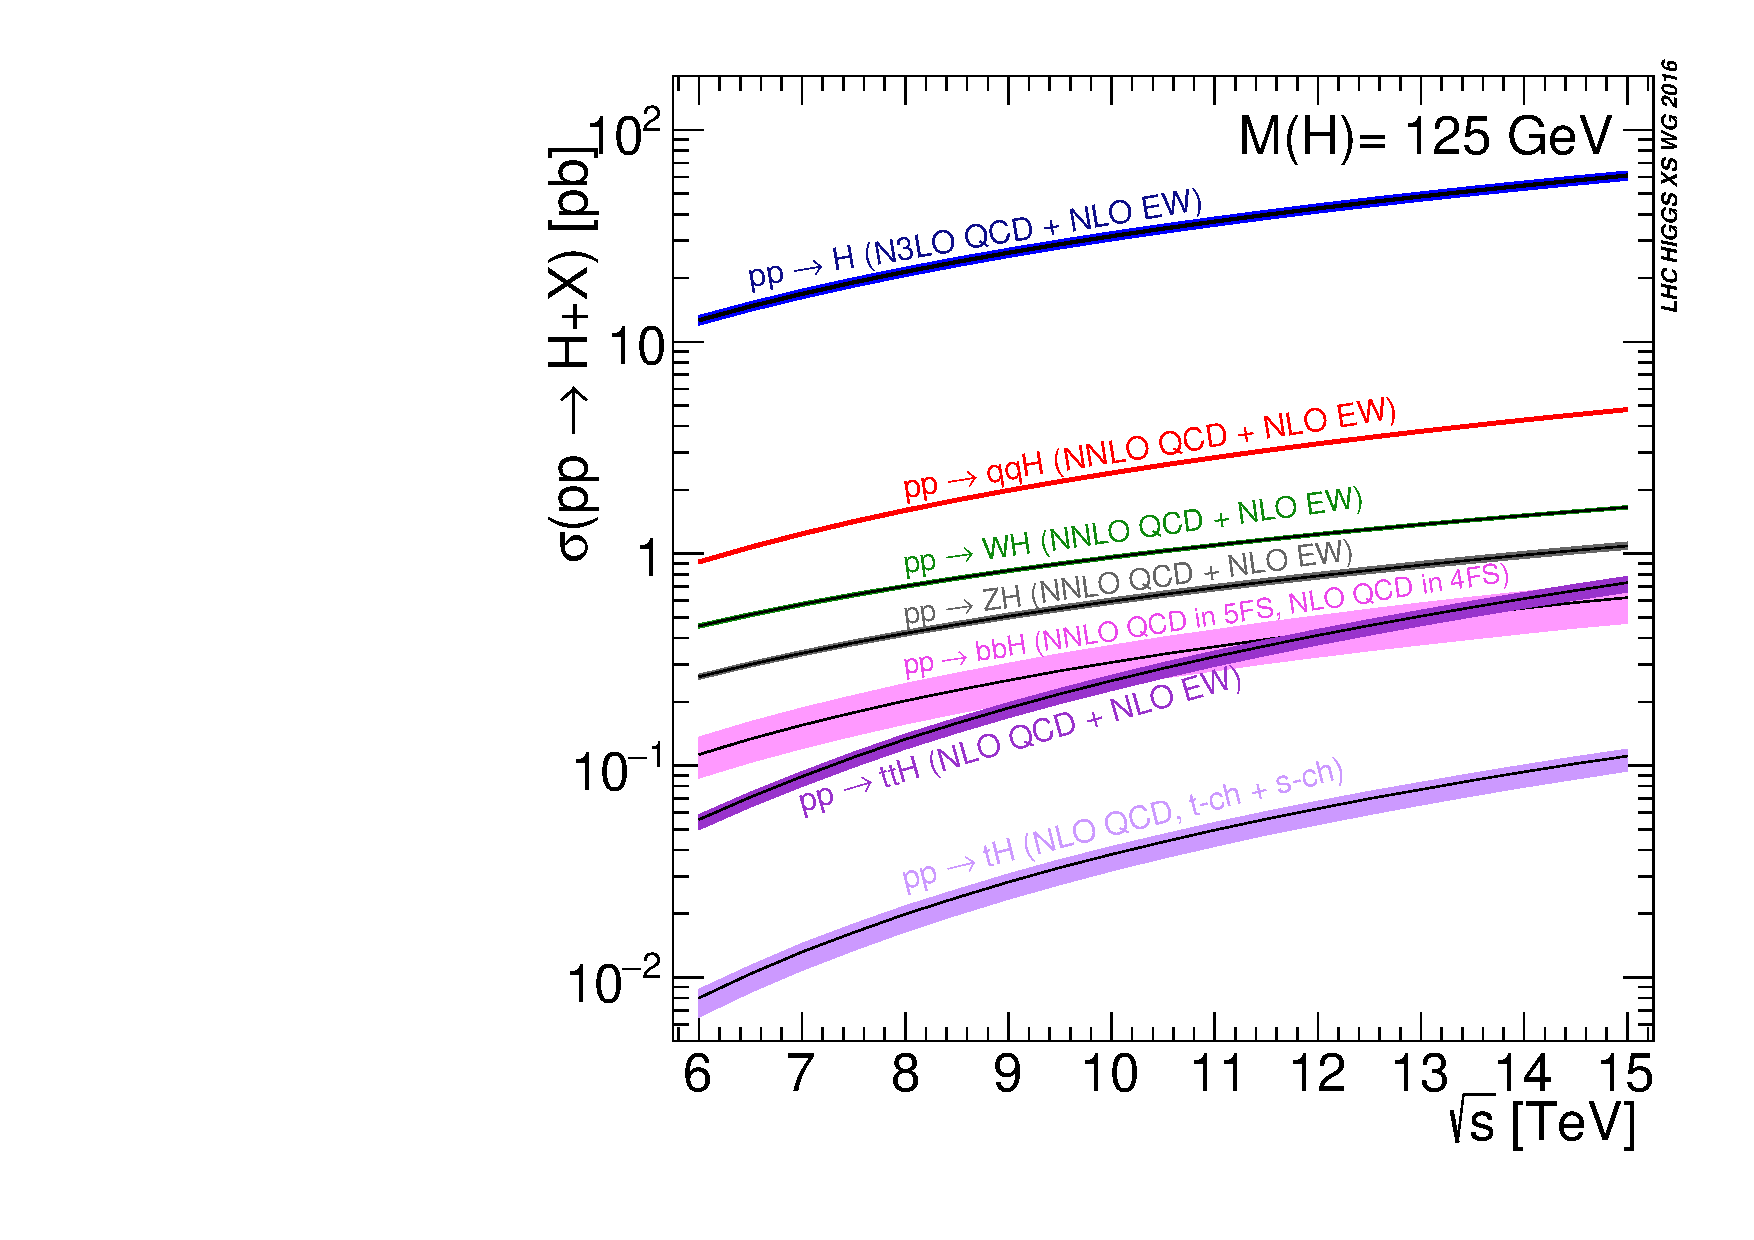
\includegraphics[width=.40\textwidth]{Plot_Escan_H125_new_sqrt.pdf}
\qquad
% "\includegraphics" from the "graphicx" permits to crop (trim+clip)
% and rotate (angle) and image (and much more)
\caption{\label{fig:a} Higg production cross-section as a function of the collison center-of-mass energy  }
\end{figure}

The Compact Muon Solenoid (CMS) is a large general purpose particle physics  detector  designed to study proton-proton collisions produced by LHC. 
\begin{wrapfigure}{r}{0.5\textwidth}
  \centering
    \includegraphics[width=.46\textwidth]{cms.png}
  \caption{\label{fig:b} The CMS detector  }
\end{wrapfigure}
A detailed description of the CMS detector can be found here~\cite{g}.
It consists of a superconducting solenoid that houses tracking and calorimetry systems and provides an axial magnetic field of 3.8T. The inner-most layer is the silicon pixel and strip tracker that measures the trajectories of charged particles and covers a range of $|\eta|<2.5$ ($\eta$ is the pseudorapidity defined as $-ln[tan(\frac{\theta}{2})]$, where $\theta$ is polar angle of the particle's trajectory with respect to the beam direction). Surrounding the tracker are the lead tungstate crystal electromagnetic calorimeter (ECAL) which measures the energy of electrons and photons, and the hadronic calorimeter (HCAL) which measures the energy of heavier particles that pass through the ECAL. The ECAL also contains preshower detector for extra spatial precision. Outside the solenoid is the muon system which has gas-ionization detectors placed in the steel yoke of the magnet. This is the outermost component of CMS and measures the momenta of muons that traverse through it.

Another vital component of the CMS is its trigger system. Only a small fraction of events produced by the LHC can be permanently stored, and to select these events of interest, CMS employs a sophisticated two-level trigger , organized in consecutive stages- the Level-1 (L1) trigger and the High Level Trigger (HLT). The L1 trigger is implemented using custom hardware and makes decisions based on coarse information from the calorimeters and the muon systems, reducing the rate from 40 MHz to 100 kHz. It has a latency of ~3.8$\mu$s. The software-based HLT partially reconstructs the event, implementing complex selection algorithms on finer granularity information from all sub-detectors in regions deemed interesting by the L1 decision. It runs on a massive computer farm and brings down the rate further to less than 1.5 kHz. I am part of a team that works on the cusp of ECAL and L-1 trigger and have helped maintain and improve the functioning of this system. This is mentioned in detail in section~\ref{sec:tech}.


\section {Overview of the Analysis}
\subsection{LFV Signal}
In BSM theories, it is possible to introduce off-diagonal Higgs-fermion Yukawa couplings such as $Y_{\mu\tau}$ in addition to the SM $Y_{\mu\mu}$,$Y_{\tau\tau}$,$Y_{ee}$ couplings allowing the Higgs to decay into to oppositely charged leptons of different flavor.  The decay studied (figure ~\ref{fig:c}) here $H\rightarrow \mu\tau$, with the $\tau$ decaying to an electron (and neutrinos) is of particular importance because CMS can much better identify and reconstruct an electron than a hadronically decaying tau making for a cleaner signature. It is important to note that $H\rightarrow \mu\tau_{e}$ final state bears some similarities with SM $H\rightarrow \tau_{\mu}\tau_{e}$ process albeit with significant kinematic differences.
\begin{wrapfigure}{r}{0.5\textwidth}
  \centering
    \includegraphics[width=.46\textwidth]{lfv.png}
  \caption{\label{fig:c} Diagram showing the LFV $H\rightarrow \mu \tau_{e}$ decay  }
\end{wrapfigure}

The muon in the LFV decay comes promptly from the H and has a harder $p_{T}$ spectrum compared to the SM muon. There are fewer neutrinos in the LFV decay which makes its missing transverse energy ($E_{T}^{miss}$) spectrum  different (neutrinos being very weakly interacting can't be detected by CMS and their transverse momenta can be estimated from $E_{T}^{miss}$, which is calculated from the imbalance in the transverse momentum of all reconstructed objects in an event ). Further, the neutrinos in the LFV process come from the decay of the highly boosted tau, leading the $E_{T}^{miss}$ and electron to be highly collinear. This fact also motivates us to use collinear mass ($M_{coll}$) as an estimator of the reconstructed H mass. This is based on the collinear approximation~\cite{h}- the mass of the H being much greater than the mass of the $\tau$, all the $\tau$ decay products are boosted in the direction of the $\tau$. The neutrino momenta ($p_{T}^{\nu,~\text{est}}$) can thus be approximated to be in the same direction of the electron and can be estimated form the projection of $E_{T}^{miss}$ onto the $\tau$ direction. The collinear mass can then be derived from the visible mass of the $\tau$-$e$ system ($M_{\text{vis}}$) as $M_{\text{col}}= M_{\text{vis}} / \sqrt{x_{\tau}^\text{vis}}$, where $x_{\tau}^\text{vis}$ is the fraction of energy carried by the visible decay products of the $\tau$ ($x_{\tau}^\text{vis}={p_{T}^{{\text{e}}}}/{(p_{T}^{\text{e}}+p_{T}^{\nu,~\text{est}})}$).

\subsection{Background processes}
Processes with final state signature same as the signal form the background processes. There are several sources of  background for this final state.
\subsubsection{$Z\rightarrow \tau \tau$}
This is the primary background for this topology where we have two tau leptons coming from the Z boson, one of which decays into an electron and other into a muon. We estimate this background using Monte Carlo simulation and validate it using a control region (CR) which is enriched in this background. This CR is constructed using kinematics cuts taking into advantage primarily the fact that reconstructed Z boson mass peaks at a much lower value than the H. We intend to improve the estimation of this background using a data driven embedding technique in the near future to estimate its shape.
\subsubsection{$t\bar{t}$}
This is a dominant background in event categories (see section ~\ref{sec:selection}) with 1 or more jets. The W leptonic decay from $t\bar{t}$ produces opposite-sign dileptons and $E_{T}^{miss}$. It is estimated using simulation and validated using a CR constructed by selecting events that have a b-tagged jet in the event thus enriching the $t\bar{t}$ contribution.
\subsubsection{Other backgrounds}
Other backgrounds include $Z\rightarrow ee,\mu\mu$  and SM $H\rightarrow \tau\tau$ decays which  are estimated using simulation.The SMH background having different kinematic characteristics than our signal is suppresed by our selection criteria described in the following section. We also have a fake background consisting of events with leptons that have been formed from misidentified particle flow (the algorithm used by CMS that combines information from all subdetectors to identify and reconstruct particles ~\cite{i}) objects in QCD and W+jets events. The fake background is small in the $\mu e$ final state and is constructed using a semi-data driven method. The W+Jets contribution is estimated using simulation with samples with different jet multiplicities being combined to improve statistical precision. The QCD multijet contribution is estimated using like-sign events in data from which the expected yields from non-QCD processes is subtracted using simulation. A like-sign to opposite-sign scale factor is then applied based on studies found in~\cite{j}. The fake background estimation is validated using a region orthogonal to the signal region that requires the electron and the muon to be loosely isolated than in the signal region enhancing the fake contribution. Other smaller backgrounds come from diboson (WW, WZ, ZZ), W$\gamma$+jets and single top-quark production and are all estimated using simulation.  


\section {Event selection}
\label{sec:selection}
In the first step of event selection a set of loose cuts is applied, the purpose of which are to provide clean events with well-defined objects and identify the basic signature. Events are required to be triggered by a loosely isolated muon with a $p_{T}$ greater than 24 GeV. An electron and muon of opposite charge separated by $\Delta R > 0.3$ (where R is the distance in the $\eta$-$\phi$ plane, $\phi$ being the azimuthal angle) must be present. Events with additional electrons, muons, or hadronic tau lepton candidates are rejected. Events with one or more b-tagged jets are rejected (this suppreses the $t\bar{t}$ background). The muon (electron) is required to have a $p_{T}$ greater than 25 (10) GeV and be within $|\eta|<2.4(2.3)$. They are also required to be tightly isolated from other objects in the event and to pass several other strict identification criterion.\\

The events are then divided into four mutually exclusive categories  based on the number of jets (with $p_{T}>30$ ,$|\eta|<4.7$ and passing a loose identification criteria). This categorization enhances different H production mechanisms and allows for category wise optimization of selection cuts increasing the overall sensitivity. The 0-jet category targets H events produced via gluon-gluon fusion. The 1-jet category primarily contains gluon-gluon fusion H events produced in association with one jet. It also contains VBF Higgs boson events where one of the jets has escaped detection. The 2-jet category is divided into two parts based on the invariant mass of the dijet system ($m_{jj}$). Events with $m_{jj}<550$ are put in the 2-jet-gg category and is targeted at gluon-gluon fusion H events produced in association with two jets. Finally, events with $m_{jj} \geq 550 GeV$ are targeted at H events produced via Vector Boson Fusion and are put in 2-jet-vbf category.\\

A stricter set of kinematic selection cuts are then applied. These cuts are meant to suppress background and optimize sensitivity( $S/\sqrt(S+B)$), where S and B are expected signal and bacground yields. The signal yield corresponds to 1\% production cross-section of the SM Higgs keeping in line with previously set limits. In the 0-jet, 1-jet , 2-jets GG and 2-jets VBF categories the transverse mass $M_{T}(E_{T}^{miss}, \mu)$ is required to be greater than 60,40,15 and 15 GeV respectively.The neutrinos from the tau lepton are expected to be approximately collinear to the electron direction so an additional requirement is made on the azimuthal angle between the electron and the $E_{T}^{miss}$;  $\Delta\phi(p_{T}^e, E_{T}^{miss}) < 0.7,0.7,0.5,0.3$ for the 0-jet, 1-jet, 2-jets GG and 2 jets VBF categories respectively. Further, in the 0(1)-jet category it is required that $\Delta\phi(p_{T}^e, p_{T}^{mu}) >2.5 (1.0)$.

\section {Multivariate analysis}
In order to improve the sensitivity of the analysis a binary classification Boosted Decision Tree (BDT) was trained to discriminate signal like events from background like events. The input data set included of simulated signal events (both from gluon-gluon Higgs and VBF Higgs mixed together) which were trained against background events from simulated $t\bar{t}$ and Drell-Yan ($Z\rightarrow \tau\tau,\mu\mu,ee$) processes mixed together. These events were all required to pass the loose selection criteria and were weighted by cross-sections of processes they come from. The training for all four categories was done combined. $t\bar{t}$ and Drell-Yan backgrounds were chosen because they together form the dominant background in all categories. Besides the $t\bar{t}$ background shares several kinematic characteristics with other smaller backgrounds such as single top and diboson. Following variables were used as BDT input:
\begin{itemize} 
\item Transverse mass between the $\mu$ and $E_{T}^{miss}$, $m_{T}(\mu, E_{T}^{miss})$.
\item Transverse mass between the e and $E_{T}^{miss}$, $m_{T}(e, E_{T}^{miss})$.
\item Azimuthal angle between the e and $\mu$, $\Delta\phi(e,\mu)$.
\item Azimuthal angle between the e and $E_{T}^{miss}$, $\Delta\phi(e, E_{T}^{miss})$.
\item Azimuthal angle between the $\mu$ and $E_{T}^{miss}$, $\Delta\phi(\mu,E_{T}^{miss})$.
\item Collinear Mass. 
\item Muon $p_{T}$.
\item Electron $p_{T}$.
\end{itemize}
Post training, the BDT score is used as a discriminant for the signal versus the background. Compared to the cut-based analysis the BDT is found to have better sensitivity.

\section {Plots and results}
The analysis is performed blinded in the signal regions and will be unblinded only when every treatment of aspect is decided and in place. Figure ~\ref{fig:plots} shows observed and predicted background comparisons for collinear mass distribution (after full cut-based selection) and BDT output distributions. The signal region is blinded. \\




\begin{figure}[htpb]
\begin{center}
\subfloat[0 jet, $M_{coll}$ distribustion]{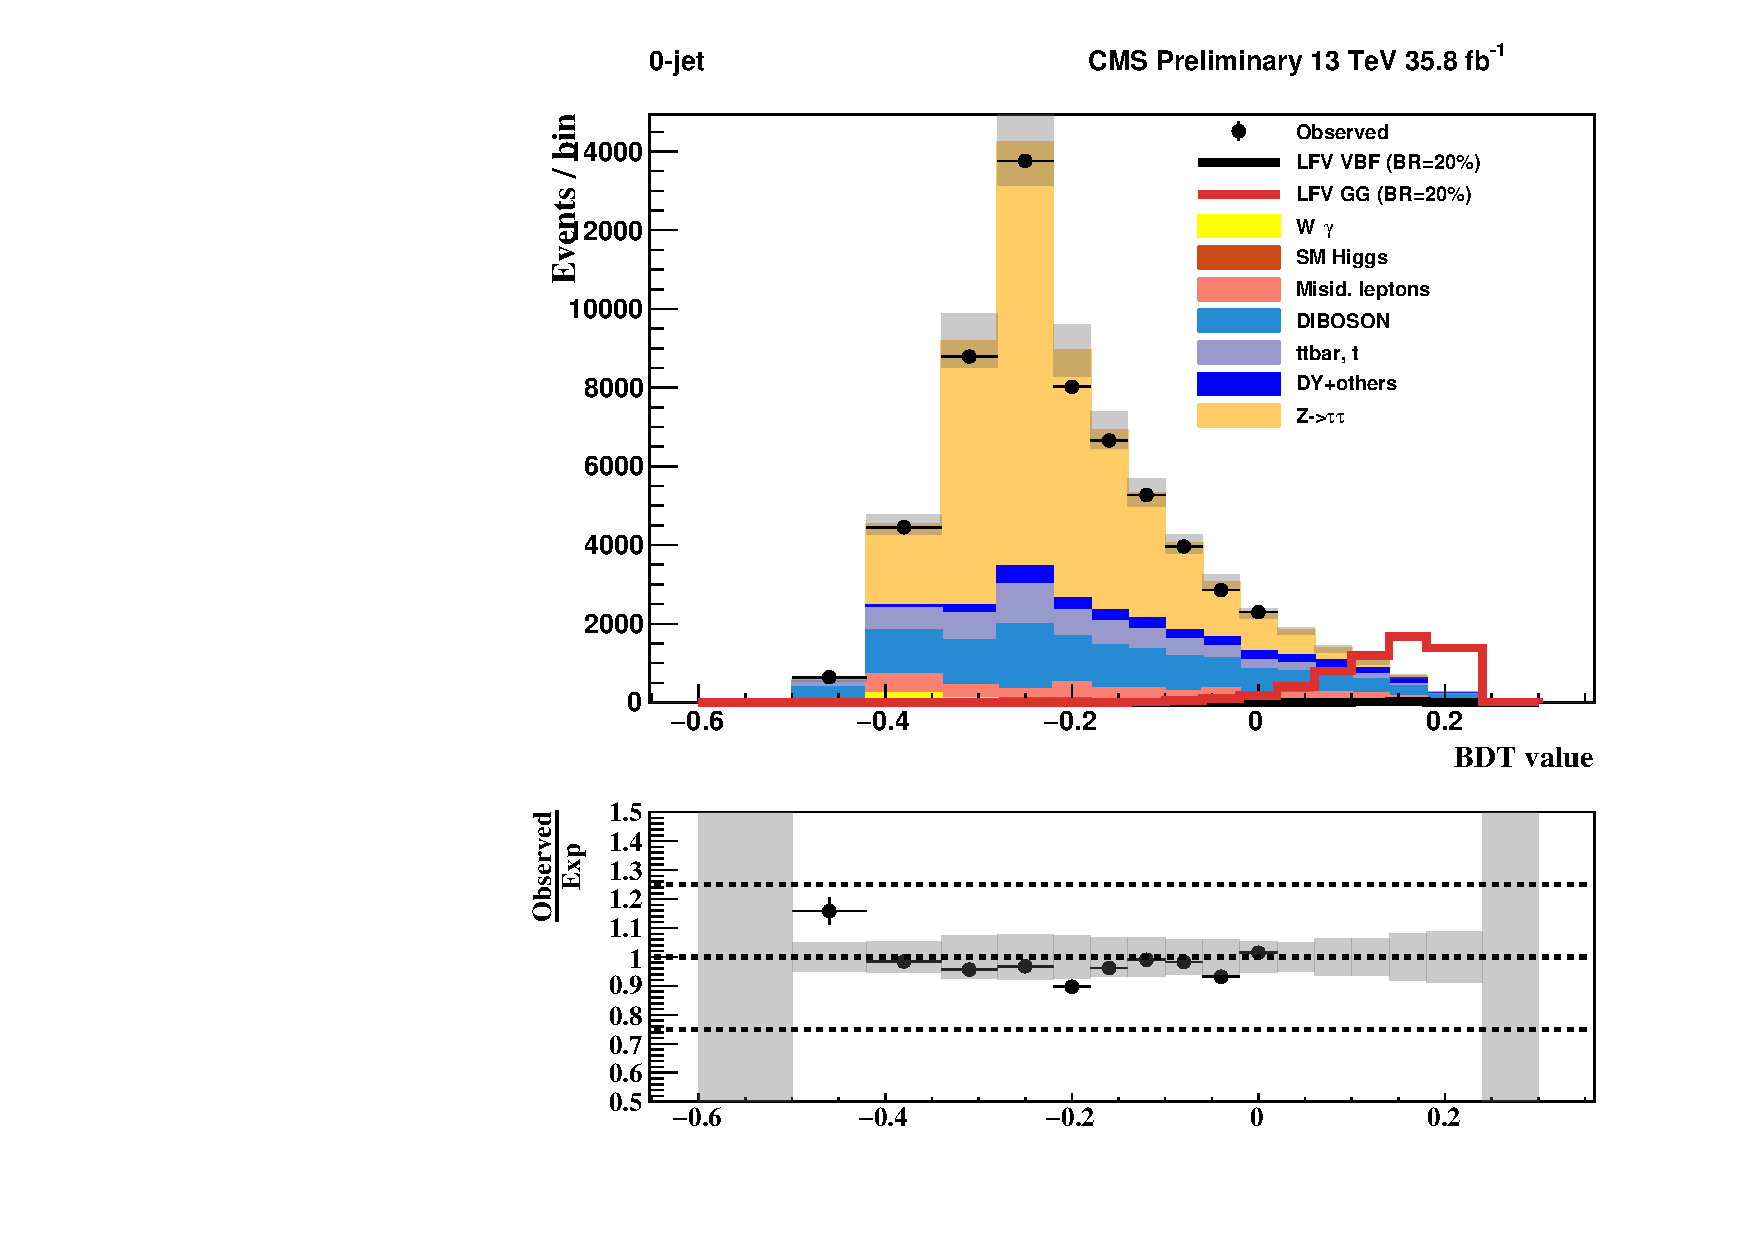
\includegraphics[width=0.30\textwidth]{0_preselection_BDT_value.pdf}}\hspace{1cm}
\subfloat[0 jet, BDT score dstribution]{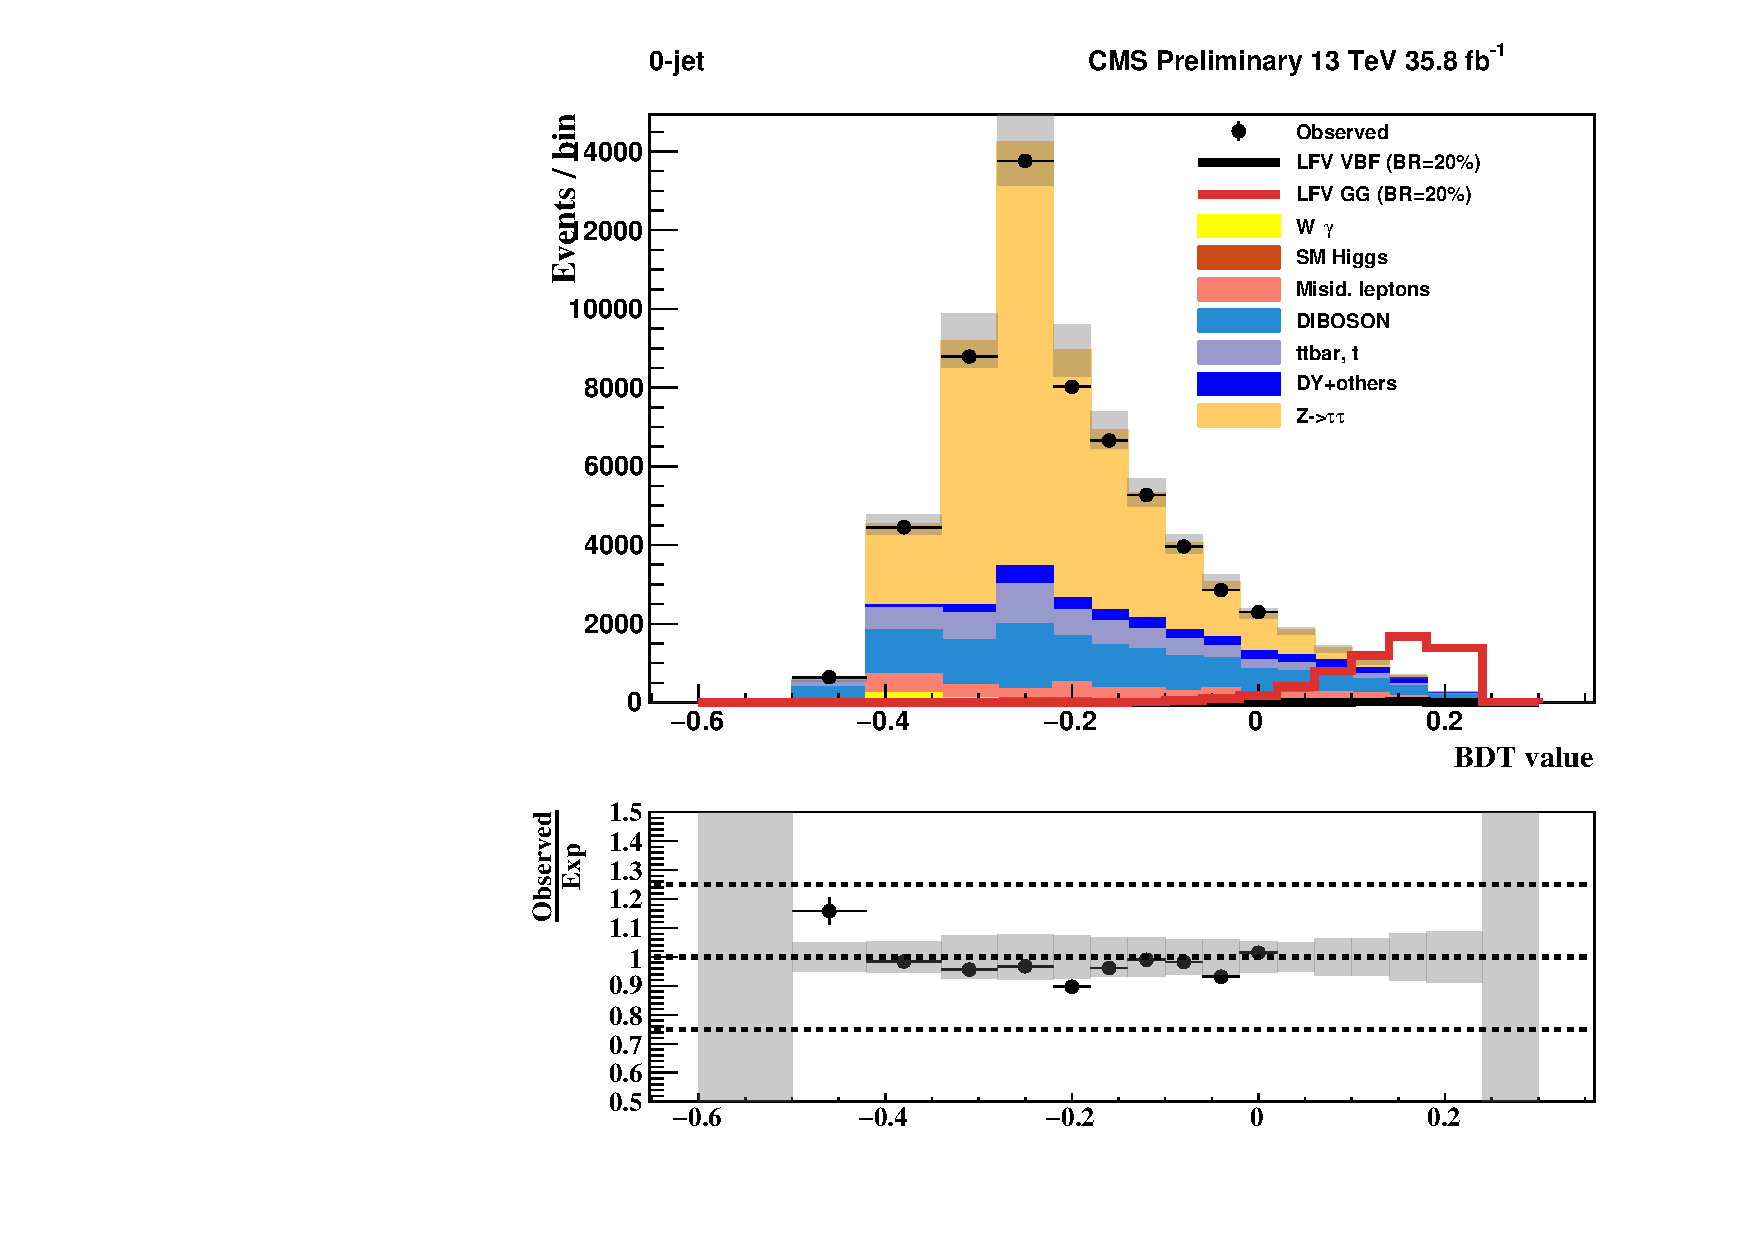
\includegraphics[width=0.30\textwidth]{0_preselection_BDT_value.pdf}}\\
\subfloat[1 jet, $M_{coll}$ distribution]{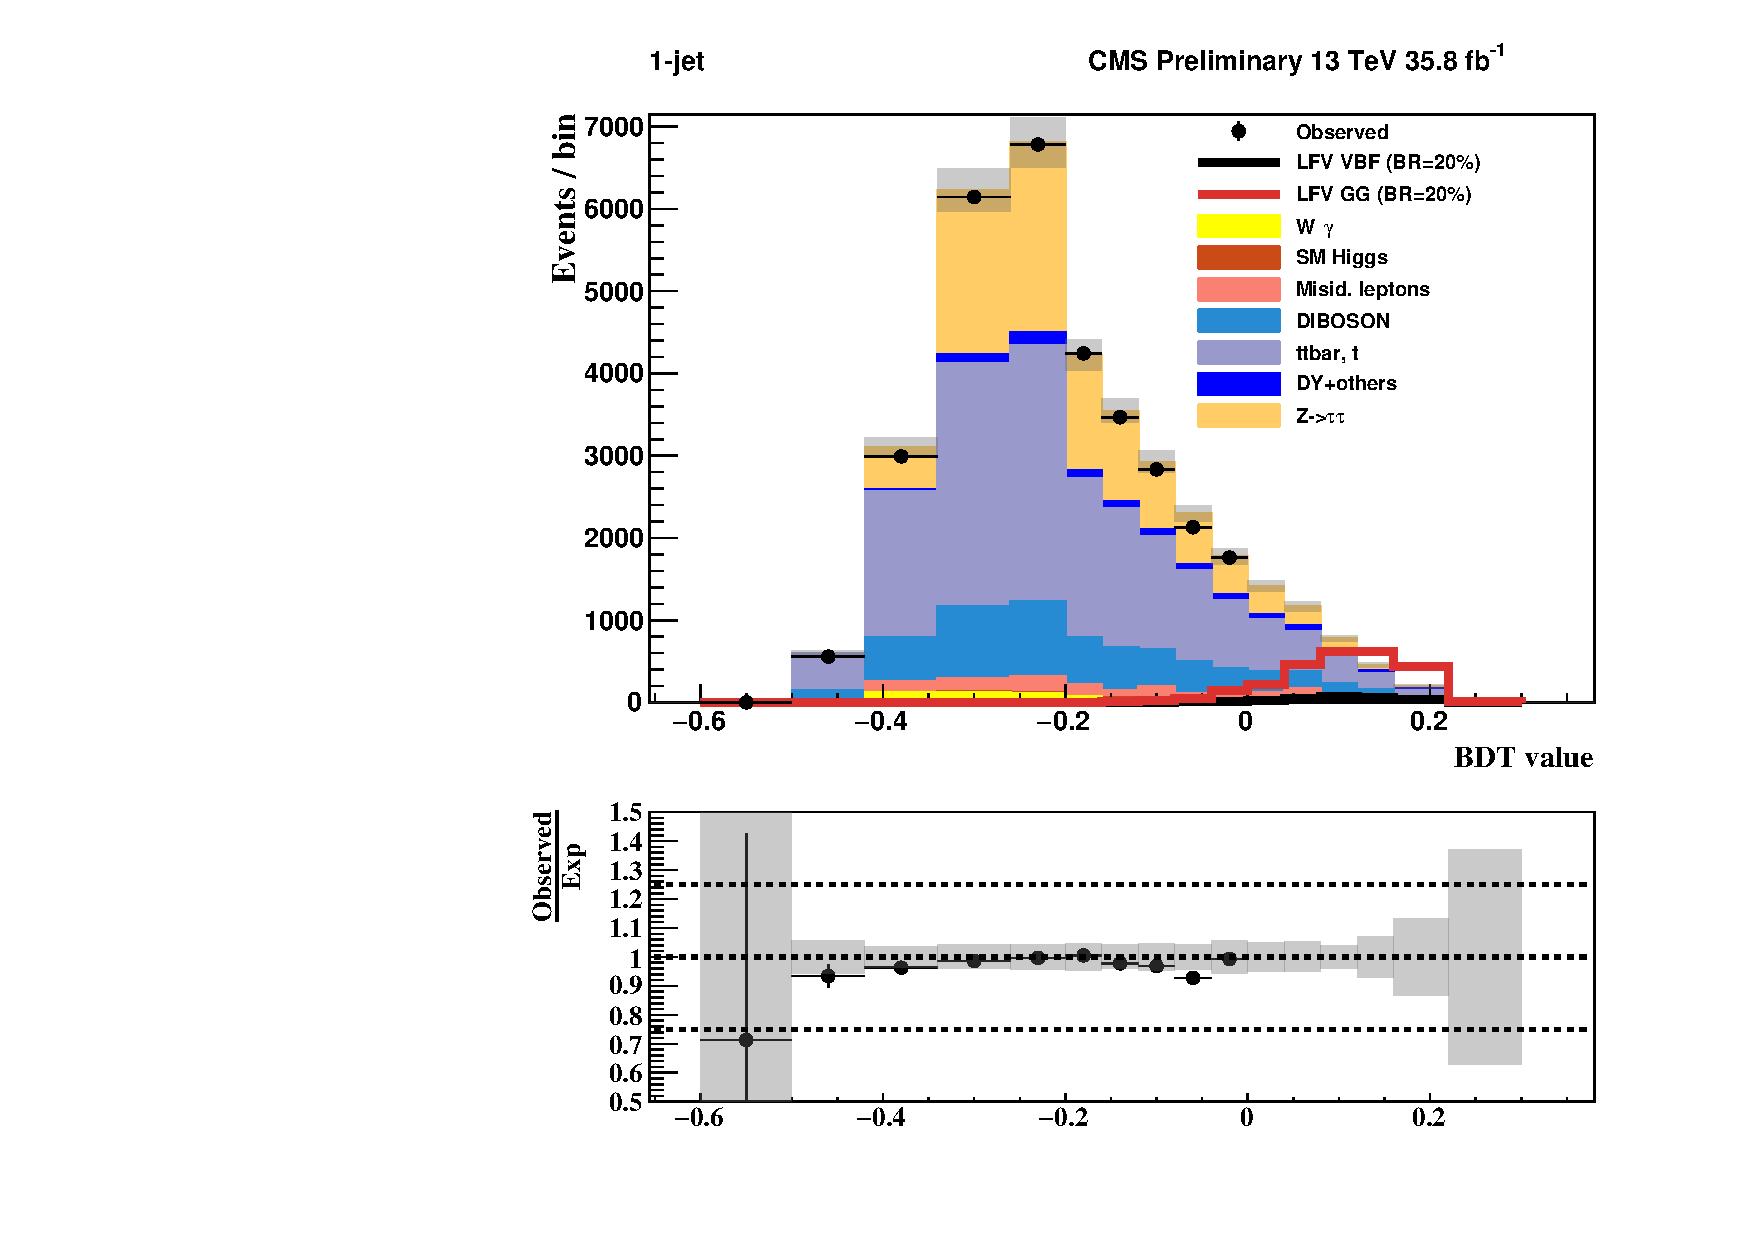
\includegraphics[width=0.30\textwidth]{1_preselection_BDT_value.pdf}}\hspace{1cm}
\subfloat[1 jet, BDT score distribution]{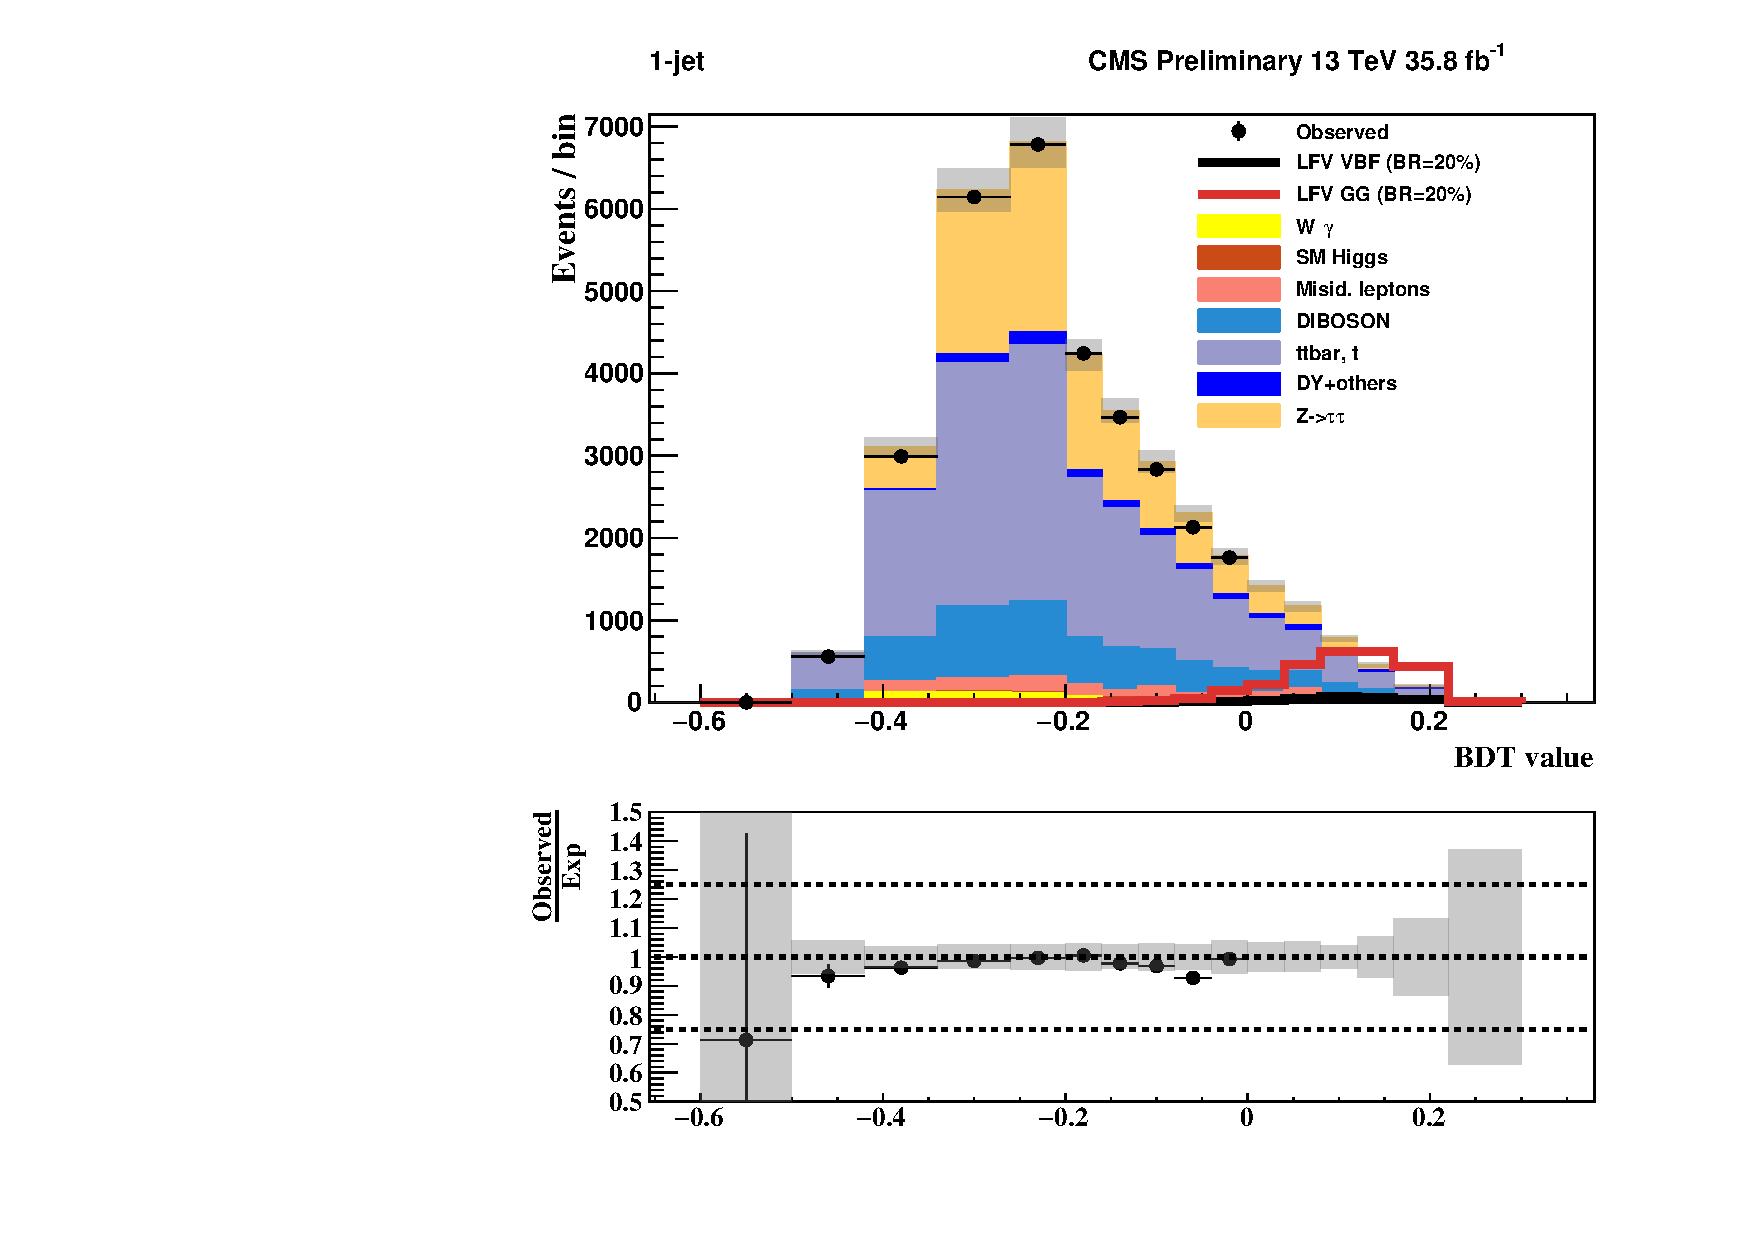
\includegraphics[width=0.30\textwidth]{1_preselection_BDT_value.pdf}}\\
\subfloat[2 jets, gg-enriched, $M_{coll}$ distribution ]{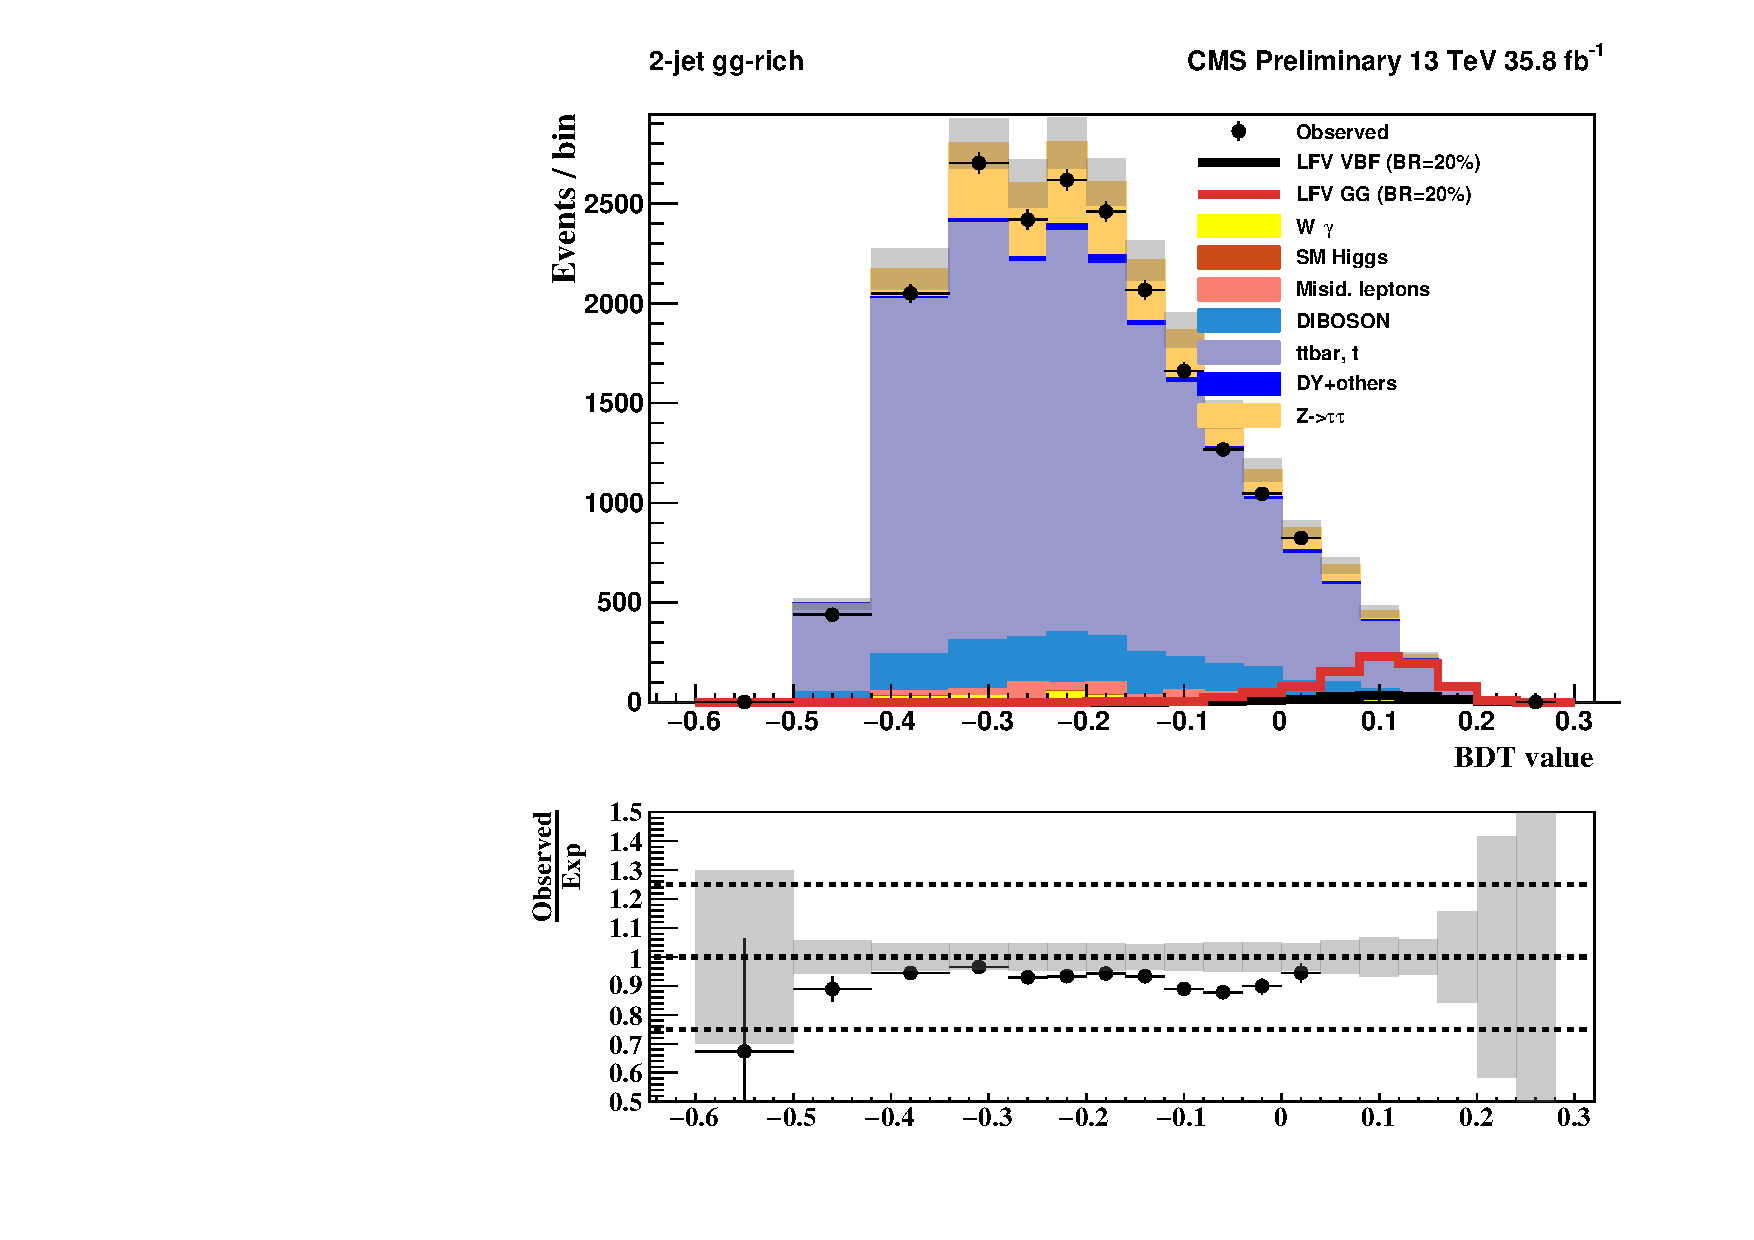
\includegraphics[width=0.30\textwidth]{21_preselection_BDT_value.pdf}}\hspace{1cm}
\subfloat[2 jets, gg-enriched, BDT score distribution ]{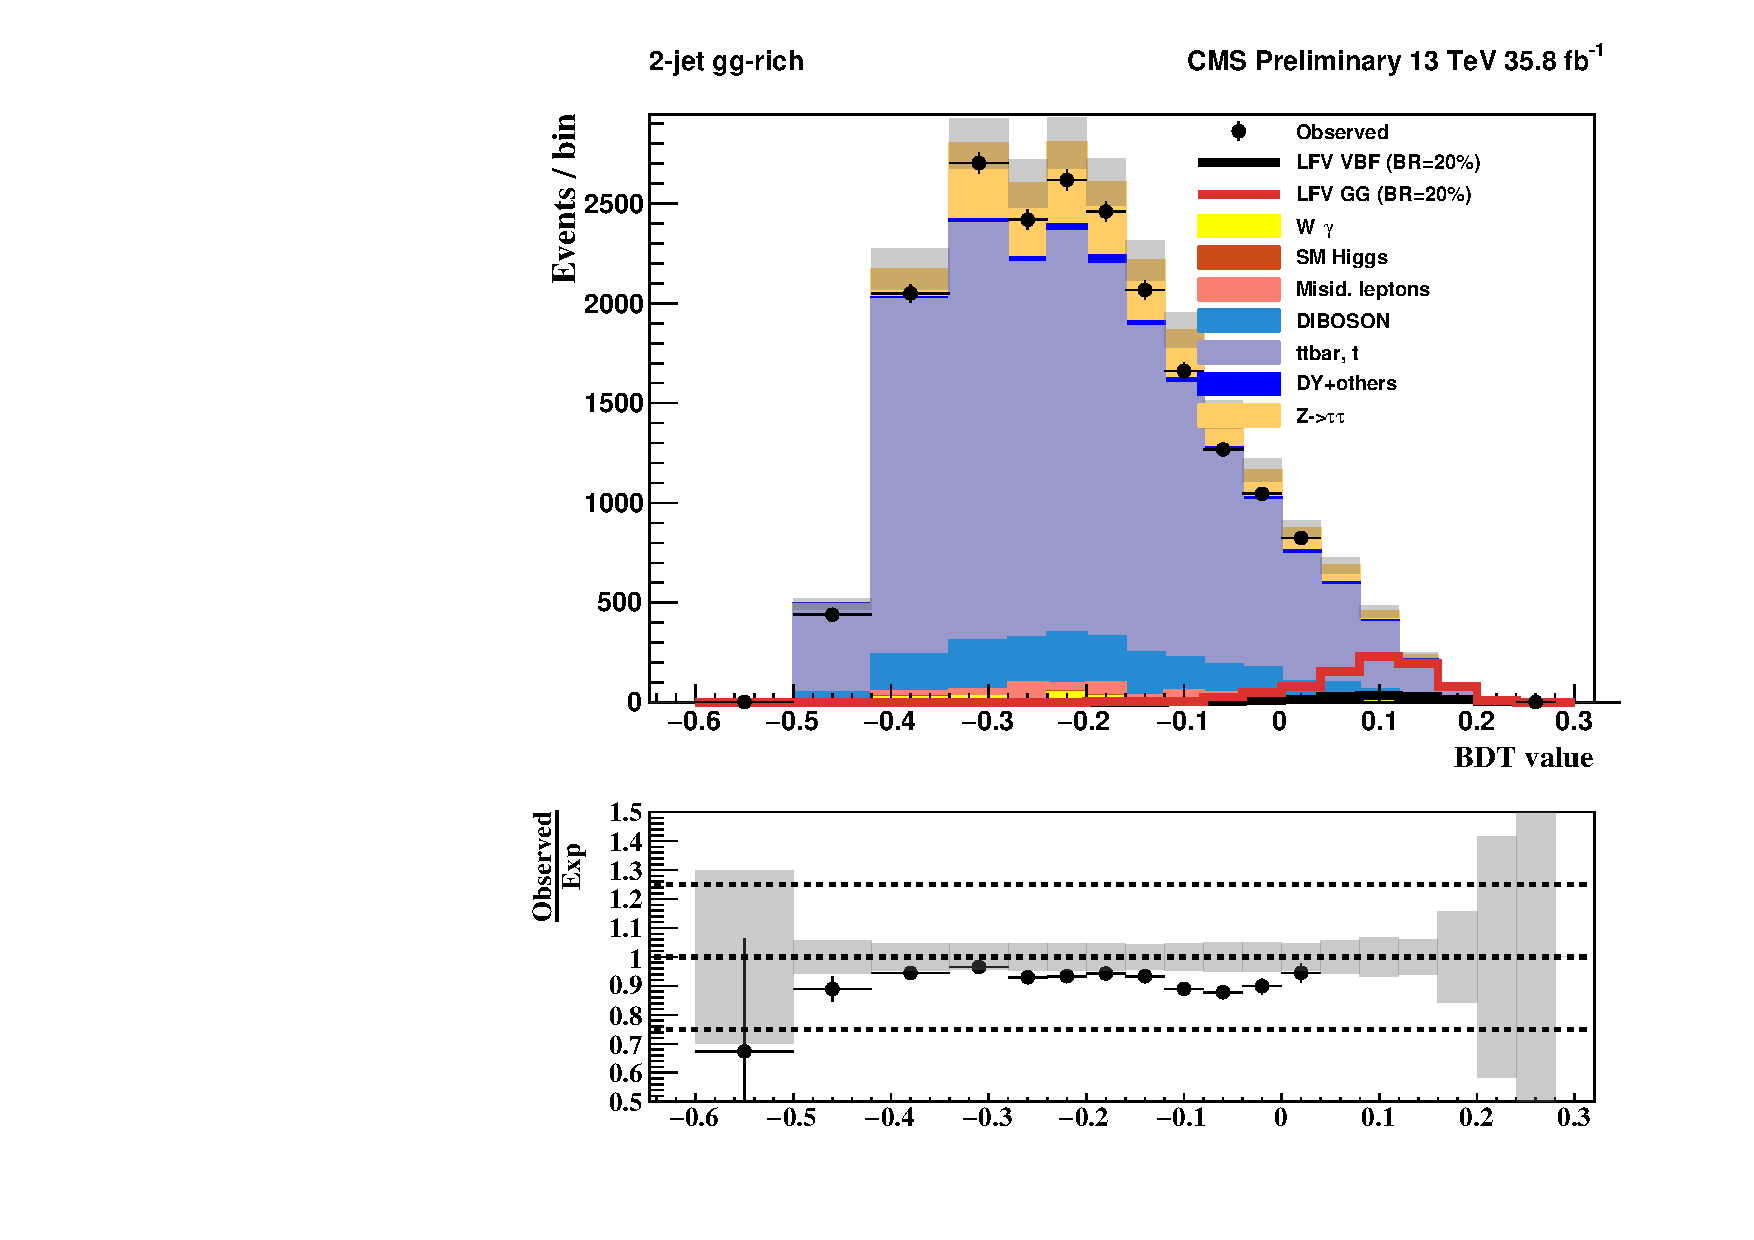
\includegraphics[width=0.30\textwidth]{21_preselection_BDT_value.pdf}}\\
\subfloat[2 jets VBF-enriched, $M_{coll}$ distribution]{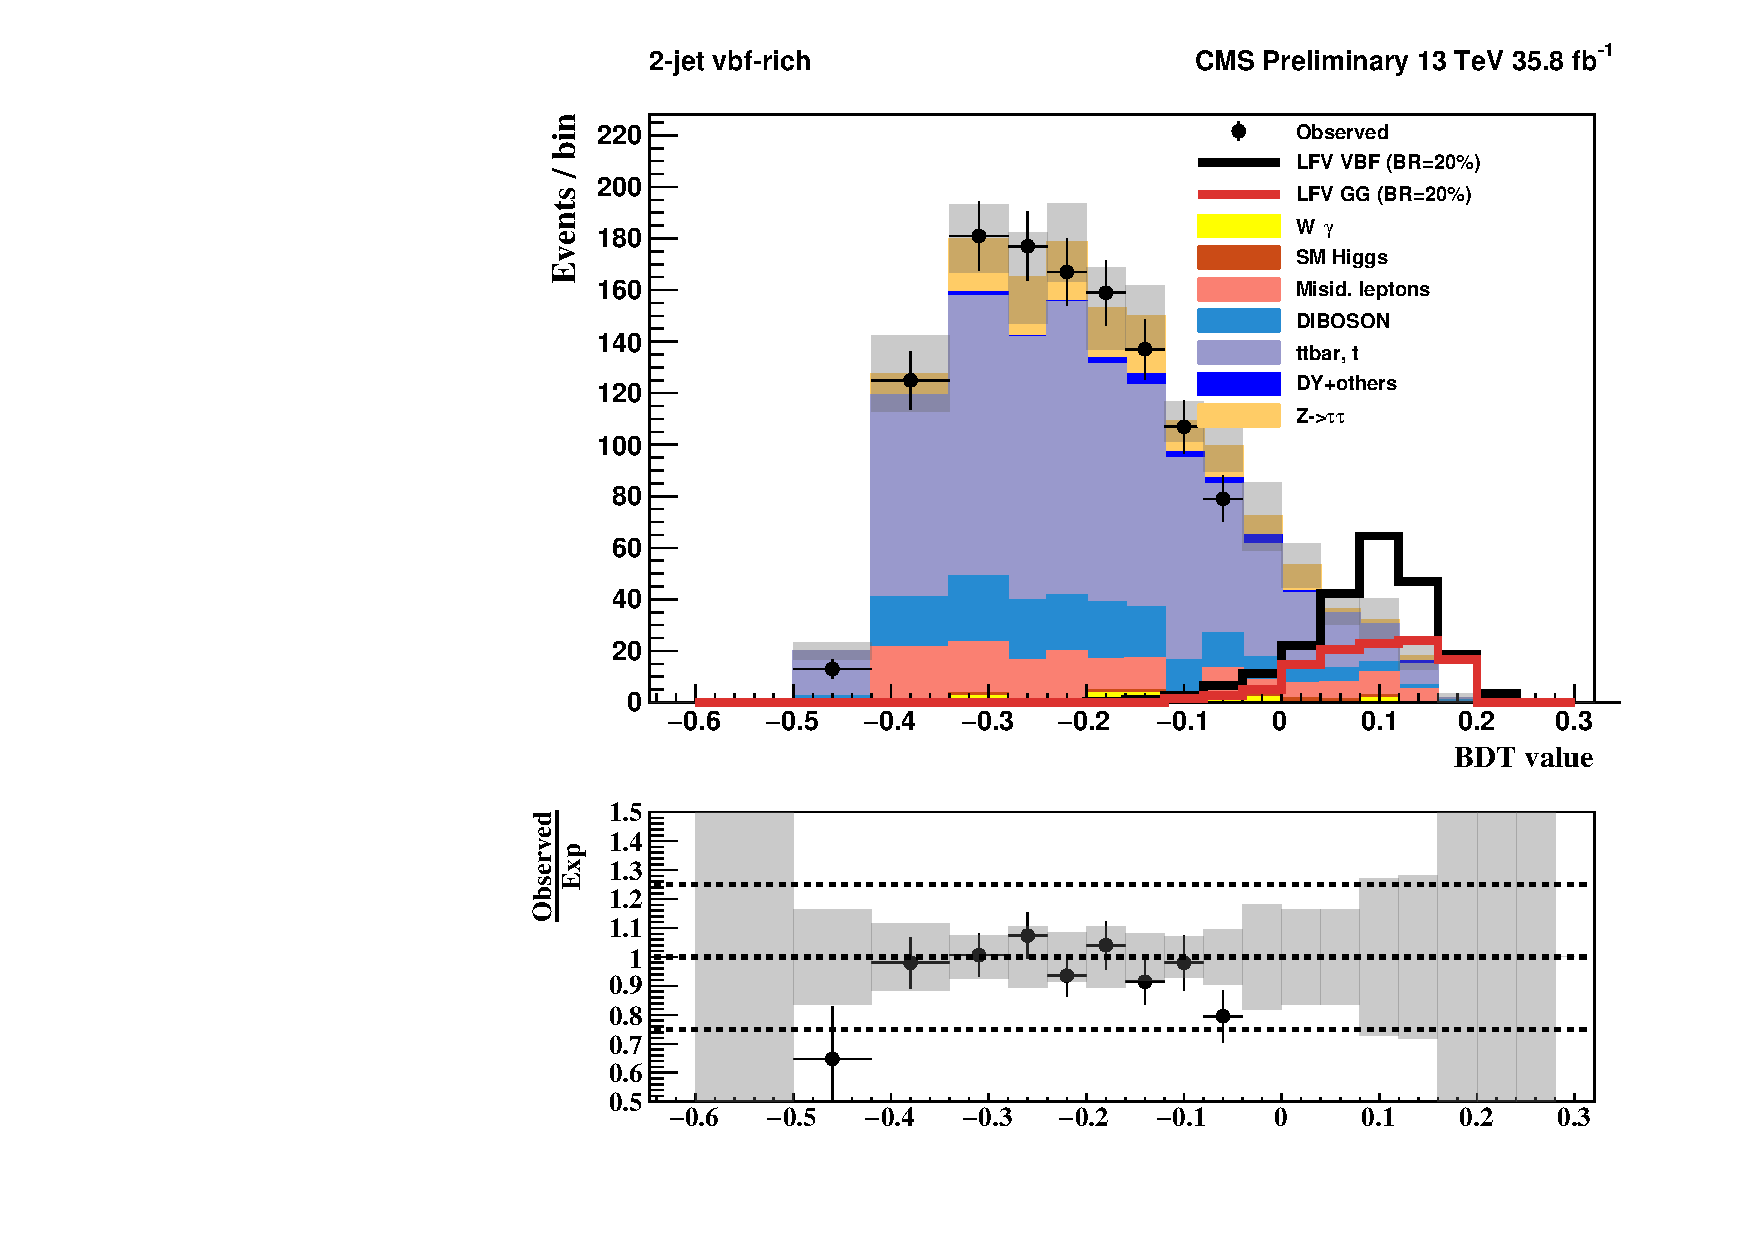
\includegraphics[width=0.30\textwidth]{22_preselection_BDT_value.pdf}}\hspace{1cm}
\subfloat[2 jets VBF-enriched, BDT score distribution]{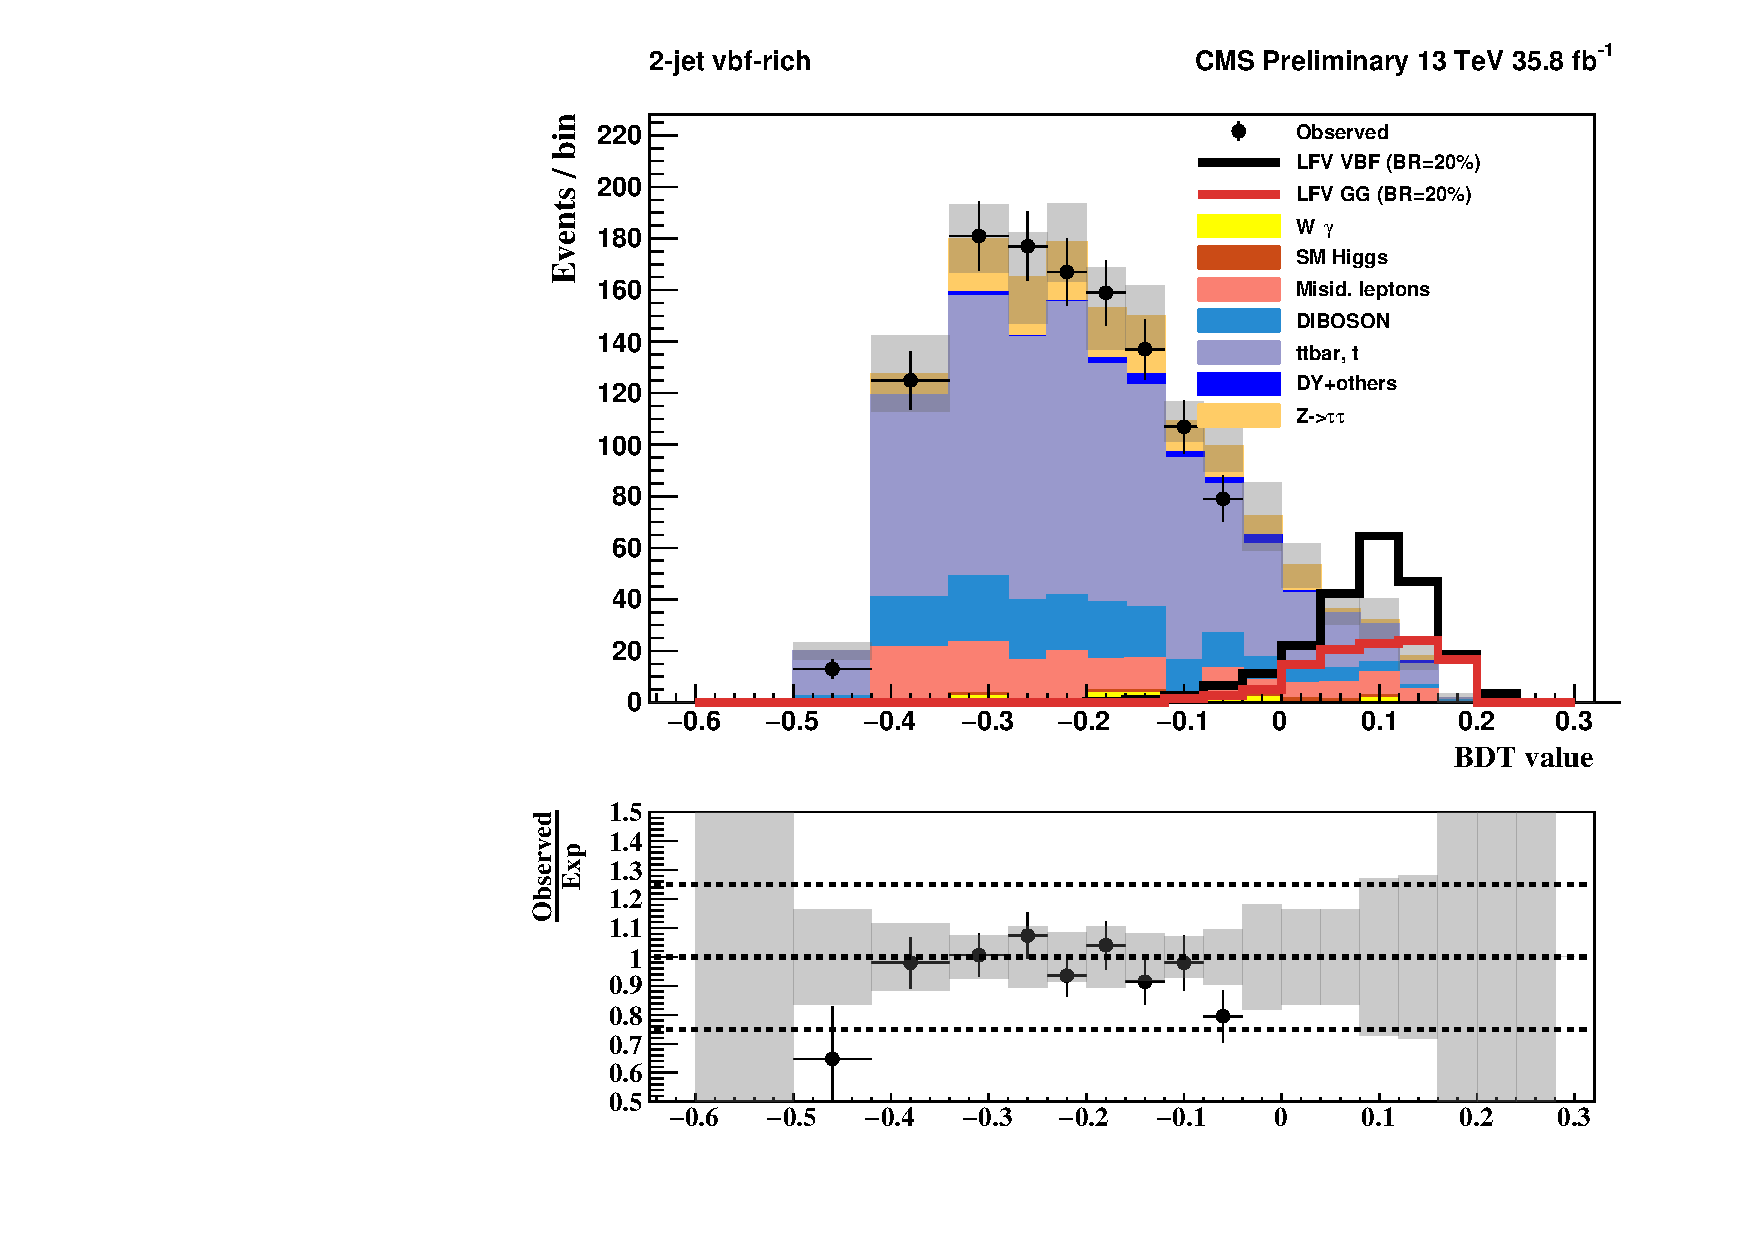
\includegraphics[width=0.30\textwidth]{22_preselection_BDT_value.pdf}}\\
\end{center}
\caption{Distributions of $M_{coll}$ after cutbased selection (left) and BDT score (right) are shown for each category. The bottom panel of each plot shows the ratio of observed yield to predicted yield in unblinded regions. The errors shown are statistical and normalization uncertainties added in quadrature. The signal yield is increased by factor of 20 for visibility.}
\label{fig:plots}
\end{figure}

A maximum likelihood fit is performed on the shape templates of signal and background binned in the discrimination variable($M_{coll}$ or BDT score). Several sources of systematic uncertainties are considered. These include uncertainties effecting only the yield/normalization that come from efficieny of trigger, identification, isolation, b-tagging, production cross-section  of simulation based backgrounds, uncertainty in the luminosity of data collected and theoretical uncertainties on the signal. We also have uncertainties that effect the shape (and normalization) of the distribution which include uncertainties coming from muon energy scale, jet energy scale, electron energy scale, unclustered energy scale and statistical bin-by-bin uncertainties.Each systematic is treated as a nuisance parameter in the fit.\\
Upper bounds on the branching fraction is set using the $CL_{s}$ method~\cite{k}. The fits are performed per category and then combined to set 95\% CL upper limits. The combined expected upper limit on $Br(H\rightarrow\mu\tau)$ for cut-based method is 0.80\%, and for the BDT based method is 0.61\%. Once the analysis is unblinded we will be able to calculate the observed limits with the 36 $fb^{-1}$ data collected in 2016. The analysis will then be either able to confirm the excess observed with run I and possibly provide evidence towards observation of a signal or will see the excess disappear. Even with lack of discovery, we will be able to place more stringent limits on the process which will guide such future searches.         

\section{Technical Contributions}
\label{sec:tech}
Other than the analysis described in the previous sections, I have been involved in some detector related projects over the past few years. I would like to particularly mention my work with CMS ECAL team which is responsible for the maintainance and improvement of the system that builds ECAL objects that are passed onto L1 trigger as inputs for combining with information from other subdetectors to make a decision to whether keep or discard the event. This system requires constant  maintainance to keep up with the more challenging conditions of the LHC and I have frequently dealt with and debugged such issues. The response of the crystals of the ECAL change over time as it is bombarded with electrons and photons. To account for this change in response a set of corrections is calculated (by the CMS laser team) every week. One of my duties has been to check and validate those corrections before they are uploaded onto our online database. Further, the barrel section of the ECAL is subjected to anomalous signals which can fake electromagnetic objects and cause us to send these fake objects to L1 causing us to lose valuable bandwidth. I have worked to improve the system dedicated to reduce such anomalous signals by tuning the parameters of the algorithm used for rejection of such signals. This tuning has to take into account several things such as effciency of identification of ecal objects and the L1 rate when attempting to reduce the percentage of these anomalous signals that pass through.\\
Besides the above,I have also been involved in simulation and test-beam studies for future upgrades of the detector. Finally, I have taken several weeklong on-call shifts at times when the detector is online, which involved intermittent monitoring of the rate coming from the ECAL, quickly dealing with problems such as bad or faulty links and generally keeping an eye on the online functioning of the system.


\begin{thebibliography}{}

\bibitem{a}CMS Collaboration, Observation of a new boson at a mass of 125 GeV with the CMS experiment at the LHC, Phys. Lett. B 716 (2012) 30.
\bibitem{b}J. D. Bjorken and S.Weinberg, Mechanism for Nonconservation of Muon Number, Phys. Rev. Lett. 38 (1977) 622, doi:10.1103/PhysRevLett.38.622.

\bibitem{c} {\bf CMS-TDR-12} (2008).J. L. Diaz-Cruz and J. J. Toscano, Lepton flavor violating decays of Higgs bosons beyond the standard model, Phys. Rev. D 62 (2000) 116005, doi:10.1103/PhysRevD.62.116005, arXiv:hep-ph/9910233.CMS Collaboration,
\bibitem{d}S. Kanemura, T. Ota, and K. Tsumura, Lepton flavor violation in Higgs boson decays under the rare tau decay results, Phys. Rev. D 73 (2006) 016006, doi:10.1103/PhysRevD.73.016006, arXiv:hep-ph/0505191.
\bibitem{e}R. Harnik, J. Kopp, and J. Zupan, Flavor violating Higgs decays, JHEP 03 (2013) 026, doi:10.1007/JHEP03(2013)026, arXiv:1209.1397.
\bibitem{df}CMS Collaboration, Search for Lepton-Flavour-Violating Decays of the Higgs Boson, Phys. Lett.B749(2015) 337–362,arXiv:1502.07400 

\bibitem{f}LHC Higgs Cross Section Working Group website, https://twiki.cern.ch/twiki/bin/view/LHCPhysics/LHCHXSWG

\bibitem{g}CMS Collaboration,The CMS experiment at the CERN LHC, Journal of Instrumentation, 3(08):S08004,2008
  
\bibitem{h}CMS Collaboration, Particle-Flow Event Reconstruction in CMS and Performance for Jets, Taus, and $E_{T}^{Miss}$ , CMS Physics Analysis Summary CMS-PAS-PFT-09-001, 2009
\bibitem{i}R. K. Ellis, I. Hinchliffe, M. Soldate, and J. J. van der Bij, Higgs decay to $\tau^{+}\tau^{-}$504 : A possible signature of intermediate mass Higgs bosons at high energy hadron colliders, Nucl. Phys. B 297 (1988) 221, doi:10.1016/0550-3213(88)90019-3.
\bibitem{j} CMS Physics Analysis Summary, Search for a neutral MSSM Higgs boson decaying into $\tau\tau$ with 12.9 $fb^{-1}$ of data at $\sqrt{s}=13 TeV$
\bibitem{k} A. L. Read, Presentation of search results: the CLs technique, J. Phys. G 28 (2002) 2693, doi:10.1088/0954-3899/28/10/313.

% Please avoid comments such as "For a review'', "For some examples",
% "and references therein" or move them in the text. In general,
% please leave only references in the bibliography and move all
% accessory text in footnotes.

% Also, please have only one work for each \bibitem.


\end{thebibliography}
\end{document}
